
%(BEGIN_QUESTION)
% Copyright 2014, Tony R. Kuphaldt, released under the Creative Commons Attribution License (v 1.0)
% This means you may do almost anything with this work of mine, so long as you give me proper credit

Explain, step by step, how to calculate the amount of current ($I$) that will go through each resistor in this series circuit, and also the current ($I$) supplied by the DC voltage source:

$$\includegraphics[width=15.5cm]{i01236x01.eps}$$

\underbar{file i01236}
%(END_QUESTION)





%(BEGIN_ANSWER)

First we need to identify all the relevant principles for series circuits:

\begin{itemize}
\item{} The algebraic sum of all voltages in the circuit will be equal to zero (Kirchhoff's Voltage Law)
\item{} Current is common throughout a series circuit, because there is only one path for current in the entire circuit
\item{} Resistances add in series
\end{itemize}

We know the voltage of the source and the resistance of the three loads.  However, we cannot simply apply Ohm's Law at this point because the source voltage is not impressed entirely on any one of the loads -- rather the source voltage will be split up proportionately amongst the three loads in accordance with KVL.  It is important to always apply Ohm's Law {\it in context}: $V = IR$ is true only if $V$, $I$, and $R$ apply to the same component or set of components.  Here, the 36 volts of the source applies to all three resistors, not to any one resistor.

\vskip 10pt

However, we may apply the principle of resistances adding in series to arrive at a total resistance value for the circuit, which we may then apply to total voltage to find total current.  Adding up the three resistors' values, we get a total resistance of $R_{total} = 1500 + 10000 + 4700 = 16200$ ohms.  Total circuit current is then calculated as follows:

$$I = {V \over R} = {36 \hbox{ V} \over 16200 \> \Omega} = 2.222 \hbox{ mA}$$

It is helpful to annotate all calculated values on the circuit schematic for easy reference.  The reason this is helpful is because it applies a context to the calculated value.  Here we will sketch arrows (in the direction of conventional flow) to document the 2.222 mA circuit current, based on the relationship between voltage and current for {\it sources} (i.e. current exits the positive pole of a source because the source is driving that current):

$$\includegraphics[width=15.5cm]{i01236x02.eps}$$

Since this is a series circuit, we know that this value of current (2.222 milliamps) will be common through all components.  Now that we know the current through each resistor and the resistance of each resistor, we may apply Ohm's Law to each resistor individually as such:

$$V_{R1} = I R_1 = (2.222 \hbox{ mA}) (1500 \> \Omega) = 3.333 \hbox{ V}$$

$$V_{R2} = I R_2 = (2.222 \hbox{ mA}) (10000 \> \Omega) = 22.222 \hbox{ V}$$

$$V_{R3} = I R_3 = (2.222 \hbox{ mA}) (4700 \> \Omega) = 10.444 \hbox{ V}$$

\filbreak

Once again it is recommended to annotate the circuit schematic with these calculated values, for the sake of keeping all calculations in context.  The polarity (+ , $-$) of each voltage is important to note as well, and we know this by the relationship between voltage and current for {\it loads} (i.e. the positive pole of a load is the one where conventional flow enters, because the voltage dropped by a load is opposing current):

$$\includegraphics[width=15.5cm]{i01236x03.eps}$$

As a final check of our work, we may sum these three resistors' voltage drops to ensure they do indeed add up to equal the source voltage in accordance with KVL:

$$ 3.333 \hbox{ V} + 22.222 \hbox{ V} + 10.444 \hbox{ V} = 36 \hbox{ V}$$
 
%(END_ANSWER)





%(BEGIN_NOTES)


%INDEX% Electronics review: series and parallel circuits

%(END_NOTES)


